\chapter{Discussione}\label{discussione}
In questa sezione verranno analizzati i risultati ottenuti dai test sulle performance del sistema illustrati nel capitolo precedente. L'obbiettivo è quello di fornire un commento sui risultati ottenuti e sulle motivazioni di situazioni anomale.

\section{SEARCH Benchmark}
Verrà effettuato un breve commento sui risultati e sui diagrammi ottenuti dai benchmark di SEARCH.

\paragraph{Metric - \texttt{measure()}}
Il benchmark visto nella Sezione \ref{section metric search} con la relativa Figura \ref{densità metric search} è quello con il maggior numero di outlier, 14/100, tutti di tipo ``severe outlier''.
\'E interessante notare dalla Figura \ref{iter-time metric search} come siano stati tutti i primi sample eseguiti a produrre questi valori particolarmente alti in un istanza di tempo circoscritta e consecutiva.
La motivazione più plausibile di questa situazione è dovuta ad un picco iniziale nella latenza di rete in quanto successivamente si trovano valori accettabili ed in linea con i restanti benchmark.

\paragraph{Contract - \texttt{evaluate()}}
Il benchmark visto nella Sezione \ref{section contract search} con la relativa Figura \ref{densità contract search}, a differenza del primo, presenta una distribuzione molto più uniforme e compatta, con tendenza ad una Normale o Gaussiana, in quanto tutti i valori tendono a concentrarsi attorno ad un singolo valore medio. \'E una distribuzione ottenibile dalla media, che ne definisce il picco centrale, e dalla deviazione standard che ne definisce la dispersione attorno ad essa.
La Figura \ref{iter-time contract search} presenta una situazione molto simile a quella del diagramma del precedente benchmark. Sono presenti outliers, più lievi dei precedenti, che però non si trovano all'inizio dell'esecuzione ma oltre il 50esimo sample.

Questa situazione avvalora maggiormente la nostra ipotesi che la fluttuazione dei risultati dei benchmark e questi outliers dipendano dalle condizioni della rete.
Se in tutti i benchmark avessimo trovato un ritardo iniziale allora la causa sarebbe stata molto probabilmente il mancato riscaldamento o la perdita dei valori in cache.


\section{SQL Benchmark}
Verrà effettuato un breve commento sui risultati e sui diagrammi ottenuti dai benchmark di SQL.

\paragraph{Metric - \texttt{measure()}}
Il benchmark visto nella Sezione \ref{section metric sql} con la relativa Figura \ref{densità metric sql} presenta anch'esso una distribuzione abbastanza compatta e simile a una Normale o Gaussiana in quanto tutti i valori tendono a concentrarsi attorno ad un singolo valore medio.
La Figura \ref{iter-time metric sql} rispetto alle due precedenti non presenta evidenza particolari di latenza tranne alcuni outliers distribuiti.


\paragraph{Contract - \texttt{evaluate()}}
Nel benchmark visto nella Sezione \ref{section contract sql} con la relativa Figura \ref{densità contract sql}, come nel caso precedente, i valori tendono a concentrarsi attorno ad un singolo valore medio
presentando una distribuzione Gaussiana.
Si può notare come la densità nella zona di outliers sia la minore rispetto a tutti i benchmark precedenti.
La Figura \ref{iter-time contract sql} presenta un'esecuzione pressoché ottima in quanto sono presenti solo due outliers e gli altri valori si condensano all'interno di un range ristretto.
\'E il benchmark avvenuto con la condizione di rete ideale.


\section{Valori anomali}\label{valori anomali}
Un'aspetto abbastanza particolare notato in entrambi i benchmark, come si può vedere nelle Tabelle \ref{benchmark search metric}, \ref{benchmark search contract} per la SEARCH e nelle Tabelle \ref{benchmark sql metric} e \ref{benchmark sql contract} per SQL, è il fatto che l'esecuzione dei metodi \texttt{evaluate()} è mediamente 1 ms più breve dell'esecuzione del metodo \texttt{measure()}.
Nei benchmark di SEARCH \textit{metric} si hanno come valori medi 6.2~ms mentre in quelli \textit{contract} si hanno 4.9 ms.
Nei benchmark di SQL \textit{metric} si hanno come valori medi 8.5 ms mentre in quelli di \textit{contract} si hanno 7.6 ms. \\
Questo risulta essere abbastanza controintuitivo e contro le nostre aspettative in quanto il metodo \texttt{evaluate()} contiene al suo intero un'invocazione al metodo \texttt{measure()} e dei controlli effettuati sui risultati; logicamente dovrebbe impiegare un tempo maggiore.

Per indagare su questi risultati sono state eseguite altre serie di benchmark. Si è notato come i valori medi di esecuzioni oscillino parecchio tra un test e l'altro riscontrando miglioramenti o regressioni fino al 50\% del valore.
Le oscillazioni si suppone ancora una volta siano dovute alla latenza introdotta dalla comunicazione di rete in quanto non si presentano in modo prevedibile nei sample.
In tutti i test successivi non si è riscontrato nulla di anomalo in merito ai tempi di esecuzione, alle statistiche e ai grafici. Si sottolinea sempre il tempo minore impiegato dalle funzioni \texttt{evaluate()}.

L'ultima prova effettuata per dare una spiegazione ai risultati è quella che ci ha fornito maggiori punti su cui riflettere.
Abbiamo provato a effettuare i benchmark con l'ordine invertito rispetto alle fasi discusse nel capitolo precedente, sono state benchate prima le funzioni \texttt{evaluate()} e poi le \texttt{measure()}. \'E stata provata questa modalità per andare a scartare l'ipotesi che dipendesse dalla cache di Elasticsearch.
Si è visto invece, al contrario di come ci si aspettava, che l'ordine con cui vengono effettuati i benchmark va ad influire sulle prestazioni medie finali, ciò è dovuto probabilmente ad un salvataggio dei valori in cache. Elasticsearch utilizza un doppio sistema di caching: da un lato si appoggia sul caching delle pagine del file-system e dall'altro sfrutta un proprio sistema di caching interno contenente i risultati delle query; il secondo benchmark dunque è lievemente favorito rispetto al primo.
Si nota come il primo metodo eseguito presenta sempre un rallentamento di qualche decimo di millisecondo.

\begin{figure}[htb]
	\centering
	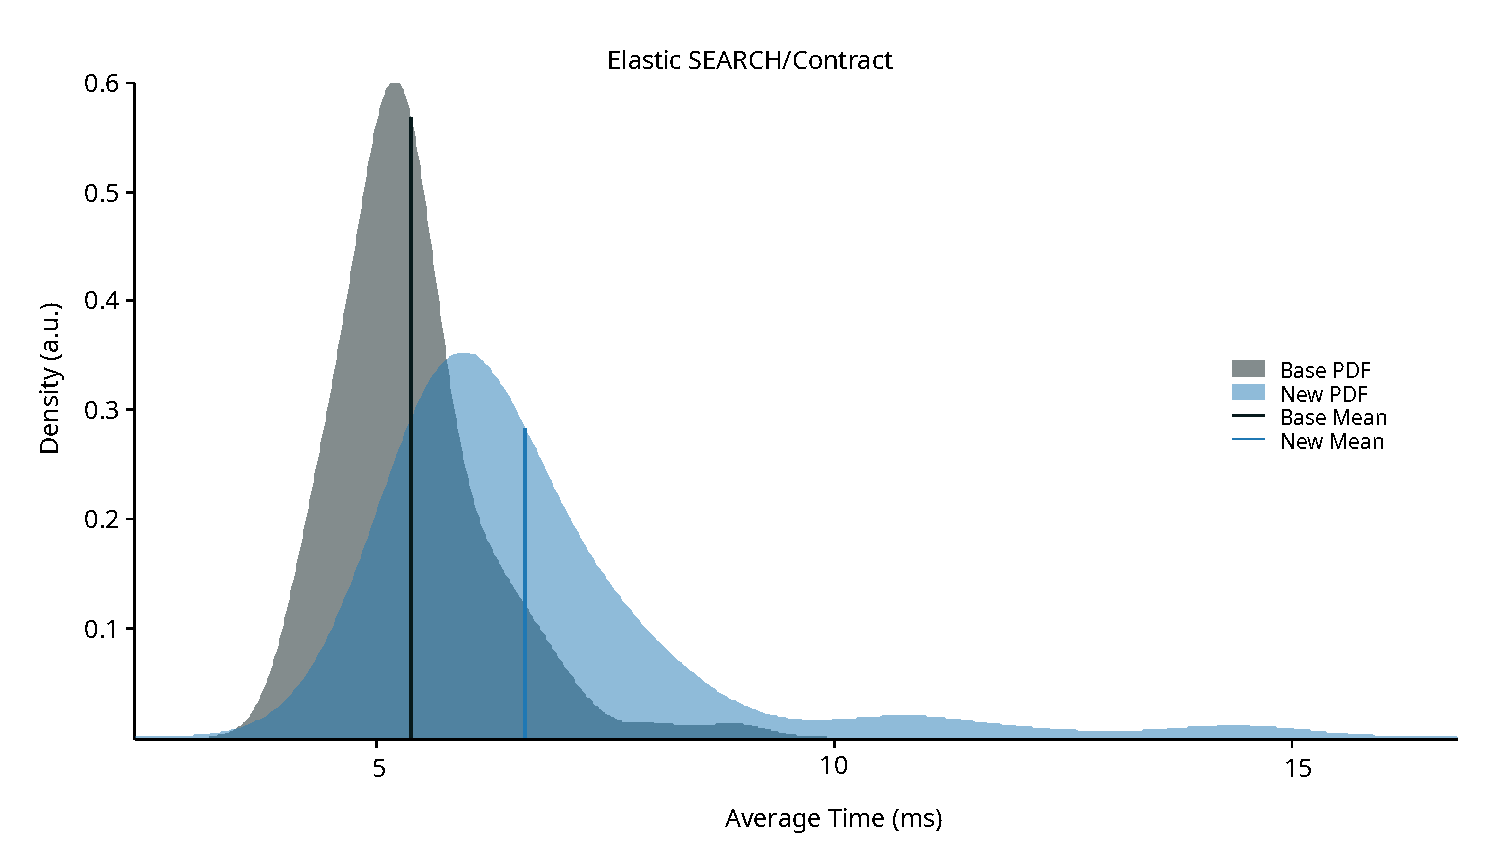
\includegraphics[width=1\linewidth]{images/benchmark/discussion/density-change.pdf}
	\caption[Diagramma confronto densità probabilistica]{Diagramma confronto densità probabilistica richieste \texttt{evaluate} di tipo SEARCH}\label{densità test}
\end{figure}

Nella Figura \ref{densità test} viene colorato di grigio la densità del metodo \texttt{evaluate()} eseguito dopo il metodo \texttt{measure()} mentre in azzurro la densità quando viene eseguito prima. Si nota come l'area azzurra è più spostata verso destra, risultando in un tempo medio lievemente maggiore.

\begin{figure}[htb]
	\centering
	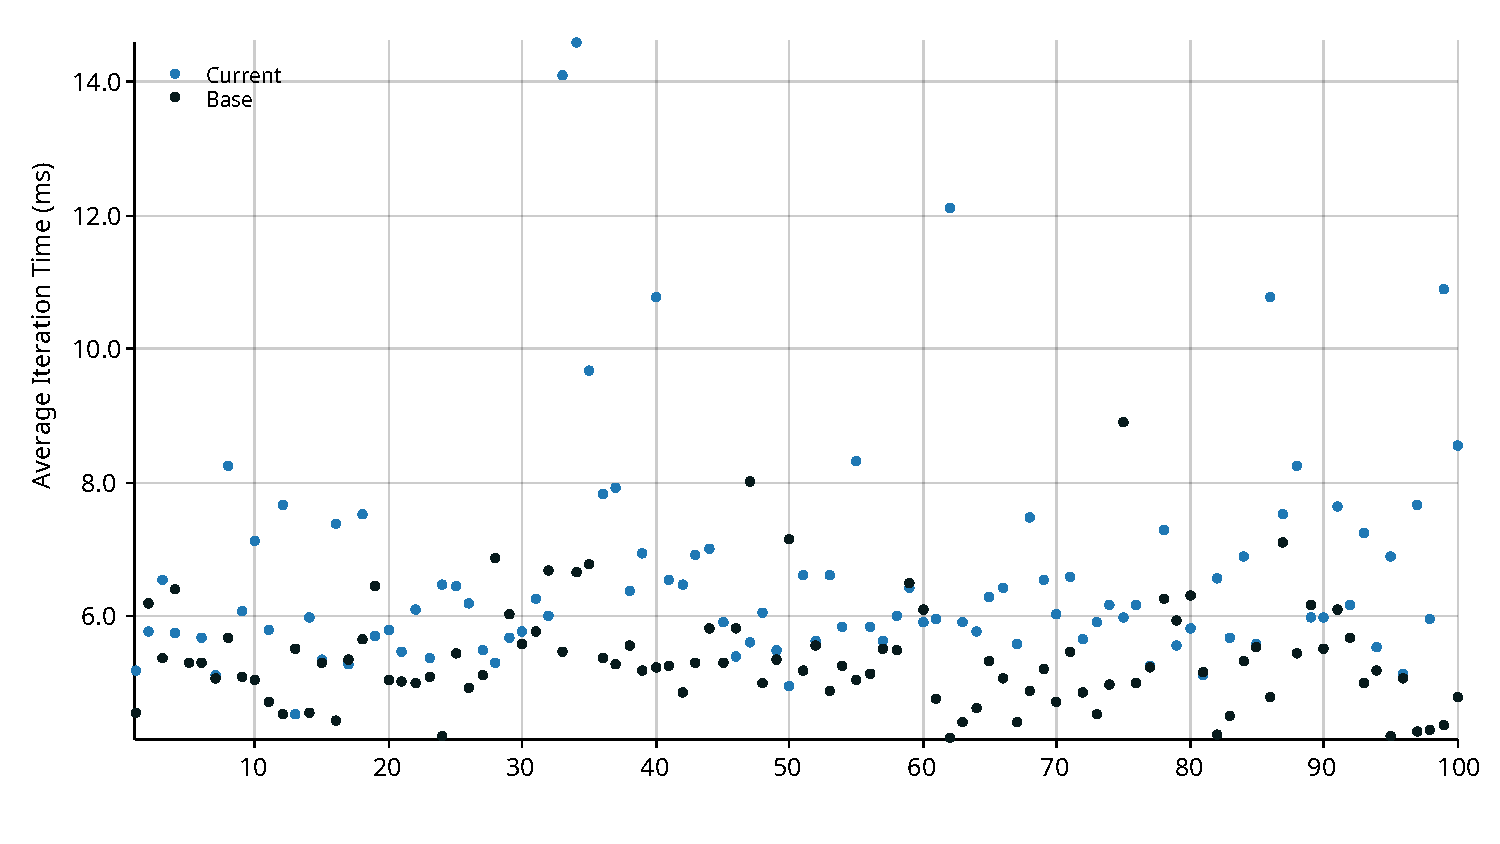
\includegraphics[width=1\linewidth]{images/benchmark/discussion/iteration-times-change.pdf}
	\caption[Diagramma confronto iteration/time]{Diagramma confronto iteration/time richieste \texttt{evaluate} di tipo SEARCH}\label{iteration-time test}
\end{figure}

La Figura \ref{iteration-time test} evidenzia lo stesso concetto mostrando però singolarmente i sample a confronto. I test in cui \texttt{contract()} viene eseguito dopo \texttt{measure()} sono rappresentati da pallini blu scuro mentre quelli eseguiti invertiti sono rappresentati da pallini azzurri. Si nota anche qua come generalmente i pallini azzurri stiano al di sopra di quelli blu.


%intendo l'overhead della cache di elastic
In conclusione, si può affermare che l'overhead introdotto dal mancato hit nella cache di Elasticsearch è talmente piccolo che risulta essere trascurabile ai fini della valutazione delle performance, mentre il fattore che causa maggiore oscillazione si dimostra quindi essere la rete e la latenza di trasmissione.
Si dimostra anche l'efficienza del sistema, sebbene effettui controlli molto semplici, e si può affermare che l'overhead introdotto dalla computazione risulta essere irrilevante rispetto a quello introdotto dalla rete.


